\documentclass[11pt,a4paper]{article}

\usepackage[margin=1in, paperwidth=8.3in, paperheight=11.7in]{geometry}
\usepackage{amsmath,amsfonts,fancyhdr,graphicx}
\graphicspath{ {img/} }
\usepackage[section,nohyphen]{DomH}
\headertitle{Internet Economics and Financial Technology - Notes}

\begin{document}

\title{Internet Economics and Financial Technology - Notes}
\author{Dom Hutchinson}
\date{\today}
\maketitle

\section{The Big Picture}

\begin{remark}{History of Commercial Computing}
  \begin{itemize}
    \item[\textit{1950-60}] Mainframes - slow; size of rooms.
    \item[\textit{1960-70}] Minicomputers - slow; couple per rooms.
    \item[\textit{1970-80}] PCs - faster; one per desk.
    \item[\textit{1980-90}] LANs - distributed networks.
    \item[\textit{1990-10}] Internet - world wide distributed network.
    \item[\textit{2010-20}] Cloud Computing
  \end{itemize}
  Where does IT go next? Has it peaked as IT is almost fully diffused?
\end{remark}

\section{Economic Principles}

\begin{definition}{Externality}
  The production or consumption of a good has an \textit{externality} if it affects a third party who was not involved in the transaction. e.g. Pollution from production is a negative externality; education is a positive externality.
\end{definition}

\subsection{Micro-Economics}

\begin{definition}{Microeconomics}
  The study of the behaviour of \underline{individual economic actors} (individuals \& business) and how decisions are made based on the allocation of limited resources.
\end{definition}

\begin{definition}{Production-Consumption Cycle}
  Producers produce goods \& services which consumers wish to buy. Consumers have a limited about of money so have to choose what to \& to-not buy at given prices. Similarly, producers have a limited number of resources (raw, labour \& capital) so need to decide what goods \& services, at what price, to produce. These lead to the idea of supply \& demand curves.
\end{definition}

\begin{definition}{Supply and Demand Equilibrium}
  The \textit{Equilibrium} of a supply-and-demand curve is a \textit{price} where the quantity demanded by all consumers is \underline{equal to} the quantity supplied by all producers.
  \par When there is \textit{excess demand} prices will rise due to scarcity of supply. The increase in supply will reduce demand as some consumers will not be happy to pay the higher price, meaning a new (higher) \textit{equilibrium price} will be reached.
  \par If there is \textit{excess supply} prices will decrease as producers try to encourage customers to buy their product over others, this will in turn attract new customers and cause some producers out of business. A new lower \textit{equilibrium price} will be reached.
\end{definition}

\begin{definition}{Consumer Demand Curve}
  A consumer's \textit{Demand Curve} plots the quantity of a product a consumer is willing to buy for a given price-per-unit. These are typically downwards sloping as consumers prefer to pay lower prices. It is assumed a consumer will buy the quantity of units equal to the point where the \textit{Demand Curve} intersects the market price.

  \par The area under the curve, but above the \textit{Market Price} is known as \textit{Consumer Surplus}. This quantifies how much more a given consumer was willing to pay than the market price. The number of items a consumer is willing to buy at the \textit{Market Price} \underline{multiplied} by the \textit{Market Price} gives the \textit{Expenditure} for that consumer. Consumers want to maximise \textit{Consumer Surplus}.

  \par See \texttt{Figure 2}
\end{definition}

\begin{figure}[ht!]
  \centering
  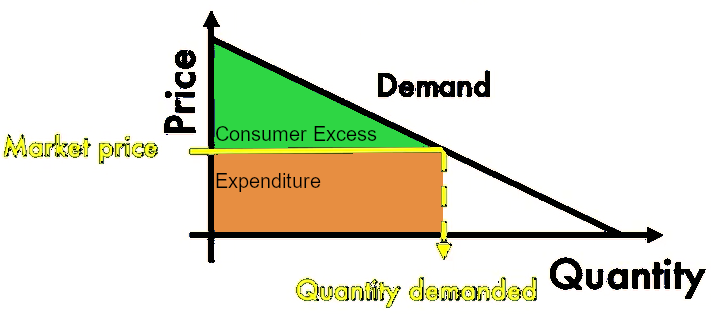
\includegraphics[width=.5\textwidth]{consumerSurplus.PNG}
  \caption{Consumer Surplus \& Expenditure}
\end{figure}

\begin{definition}{Production Costs}
  A producer will have costs they need to pay in order to stay in business. These costs can be categorised as
  \begin{itemize}
    \item[\textit{Fixed Costs}] A company must incur in order to operate, even before they start producing. (e.g. rent)
    \item[\textit{Variable Costs}] are costs which depend on the number of units produced. (e.g. equipment, raw materials)
    \item[\textit{Semi-Variable Costs}] Labour can be considered a variable cost as you can choose to pay overtime or to hire someone new in order to increase production.
  \end{itemize}
  The sum of these values will give you the \textit{Total Cost} of production.
\end{definition}

\begin{definition}{Marginal Cost Curve}
  \textit{Marginal Cost} is the cost of producing the \underline{last} unit. It is equal to
  \[ \dfrac{\text{Change in Cost}}{\text{Change in Quantity Produced}} \]
  \par We can plot a \textit{Marginal Cost Curve} of marginal cost against quantity. Typically these are initially downwards sloping, then upwards sloping.
\end{definition}

\begin{definition}{Economies of Scale}
  When the \textit{Marginal Cost Curve} is downwards sloping \textit{Economies of Scale} are being experienced. \textit{Economies of Scale} are the cost advantages a producer obtains by scaling their business. e.g. By hiring a new staff member existing staff are able to specialise better on their task and thus production per staff member increases.

  \par When the \textit{Marginal Cost Curve} is upwards sloping \textit{Diminishing Marginal Returns} are being experienced. This is common as it is unlikely that hiring 10 new staff will increase marginal production by 10 times that of a single new staff member.

  \par Economies of scale \& diminishing marginal returns affect the \textit{Cost Curve} for a producer.
\end{definition}

\begin{remark}{Minimum Sale Price}
  The \textit{Marginal Cost} of a product is the minimum price a product must be sold at in order to make a profit.

  \par A producer will go out of business if it cannot sell above its \textit{Average Variable Cost} (per unit produced) in the \underline{short run}; and if cannot cover its \textit{Average Total Cost} (per unit produced) in the \underline{long run}.

  \par The point where these \textit{AVC} \& \textit{ATC} curves intersect the \textit{Marginal Cost Curve} define the minimum amount of units a business needs to sell to stay in business in the short and long term, respectively.
\end{remark}

\begin{figure}[ht!]
  \centering
  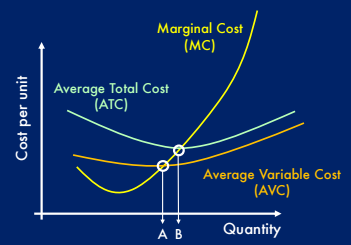
\includegraphics[width=.5\textwidth]{physicalCostCurve.PNG}
  \caption{Cost Curve for a Product of a Physcial Retailor}
\end{figure}

\begin{definition}{Business Supply Curve}
  A business's \textit{Supply Curve} is the minimum price-per-unit it is willing to sell each quantity of product at. It tends to be upwards sloping as marginal cost increases with quantity. The \textit{Supply Curve} will be truncated and not have a value for small quantities (in practice) as the business would fail if it sold too few products.
\end{definition}

\begin{definition}{Market Supply Curve}
  The \textit{Market Supply Curve} is the total number of units available, for a given price, across all producers in a market.

  \par The area above the \textit{Market Supply Curve} and below the \textit{Market Price} is the \textit{Producer Surplus}. This is the total additional income a producer receives after costs (i.e. total profit). Producers want to maximise \textit{Producer Surplus}
\end{definition}

\begin{definition}{Competitive Equilibrium}
  In a \textit{Competitive Market} the \textit{Market Equilibrium Price} will be that where the \textit{Consumer Demand Curve} and \textit{Market Supply Curve} intersect, as this is the price where quantity demanded and supplied are equal. The \textit{Market Equilibrium Price} maximises total surplus for both consumers and producers.
\end{definition}

\begin{definition}{Shifts}
  \textit{Shifts} can occur which move the whole of a supply or demand curve. These occur from non-price factors. e.g. a pandemic will cause a shift in the demand curve for face masks. These will cause a shift in  \textit{equilibrium price}.
\end{definition}

\begin{definition}{Monopoly Market}
  A market is considered a \textit{Monopoly} if its structure is characterised by a single seller (The \textit{Monopolist}). The \textit{Monopolist} faces no competition and thus can be a price \underline{setter}, rather than price taker. In the real world a firm with over 40\% market share is considered to have a monopoly. Monopoly markets are not competitive.
\end{definition}

\subsection{Elasticity}

\begin{definition}{Price Elasticity of Demand}
  \textit{Price Elasticity} is a measure of the how much the price of a product affects the quantity demanded. The more horizontal the demand curve, the greater the quantity demanded increases for a given decrease in price, (i.e. the more elastic the price is).
  \begin{itemize}
    \item A \textit{Horizontal} demand curve has \textit{Perfect Price Elasticity} as a change in quantity has no affect on price.
    \item A \textit{Vertical} demand curve has \textit{Perfect Price \underline{In}elasticity} as a fix quantity is demanded, at any price.
    \item A \textit{45 degree} demand curve has \textit{Unit Price Elasticity} as an $\Delta\%$ change in supply will produce an $\Delta\%$ change in demand.
  \end{itemize}
\end{definition}

\begin{definition}{Price Elasticity of Supply}
  \textit{Supply Elasticity} is a measure of how much a change in quantity supplied will affect the cost of production. The more horizontal the \textit{Supply Curve} is the less the price of production increases for a given quantity.
  \begin{itemize}
    \item A \textit{Horizontal} demand curve has \textit{Perfect Price Elasticity} as a change in quantity has no affect on price.
    \item A \textit{Vertical} demand curve has \textit{Perfect Price \underline{In}elasticity} as a fix quantity is demanded, at any price.
    \item A \textit{45 degree} demand curve has \textit{Unit Price Elasticity} as an $\Delta\%$ change in supply will produce an $\Delta\%$ change in demand.
  \end{itemize}
\end{definition}

\section{The Economics of The Internet}

\begin{definition}{Network Externalities}
  A \textit{Network Externality} is an \textit{Externality} that occurs when the act of buying a product/serivce has an indirect cost or benefit to those who already own the same product/service. Products with \underline{positive} network externalities are often known as \textit{Network Goods}.

  \par Owning a mobile phone has a positive network externality as you are increasing the number of contactable people. Owning a car has a negative network externality as you increase road traffic.

  \par Positive network externalities can produce a \textit{Positive Feedback Loop} where people by products which are compatible with their friends, rather than necessarily the best product. This is part of \textit{Brand Value}.
\end{definition}

\begin{definition}{Network Effect Demand Curve}
  We can plot a \textit{Network Effect Demand Curve} (\texttt{Figure 3}) of the price customers are willing to pay against network size. This is slope upwards initially as the marginal value of each extra user is higher; eventually it will slope downwards as these marginal gains diminish.

  \par For any given price there are three equilibrium points $q_0,q_1,q_2$ for network size. $q_1$ is deemed unstable, the \textit{`tipping point'}, as once the network is larger than $q_1$ it will naturally grow to $q_2$ (as there is a consumer excess) but whilst it is smaller it will shrink to $q_0$ (as there is a consumer deficit). This means $q_1$ is the \textit{Critical Mass} for the network to be sustainable.
\end{definition}

\begin{figure}[ht!]
  \centering
  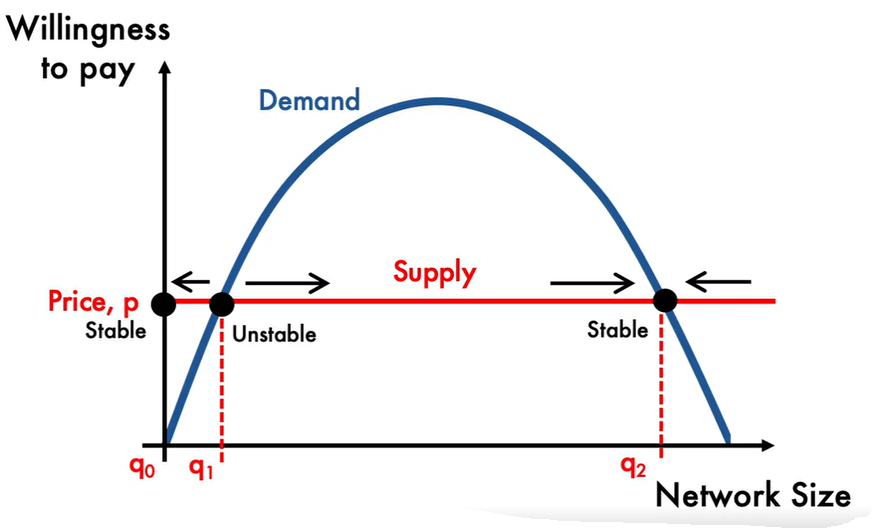
\includegraphics[width=.5\textwidth]{networkDemandCurve.PNG}
  \caption{Network Effect Demand Curve}
\end{figure}

\begin{proposition}{The Long Tail}
  Sales business typically sell either: high volume, low margin goods (e.g. burgers); Or, low volume, high margin goods (e.g. cars). Physcial sales businesses are constrained by the physical shelf space they have and thus avoid low volume, low margin goods. This means that the sales distribution for products in a physical store will be a truncated \textit{Pareto Distribution}.\\
  \par Internet businesses have unlimited shelf space to advertise products, and since warehouse space is much cheaper (per sq ft) they can store a lot more products for the same cost, effectively increasing the margin of each product. Meaning their are more products which are profitable to stock and the sales distribution for products of an internet business will have a much longer tail. (See \texttt{Figure 1}).
\end{proposition}

\begin{figure}[ht!]
  \centering
  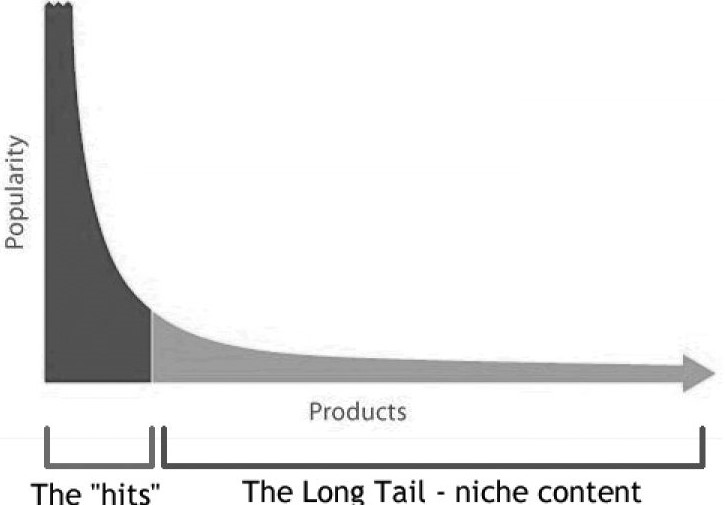
\includegraphics[width=.5\textwidth]{LongTail.jpg}
  \caption{The Long Tail}
\end{figure}

\begin{remark}{How to take advantage of `The Long Tail'}
  \begin{enumerate}
    \item Make everything available.
    \item Reduce prices (due to economies of scale \& reduced costs).
    \item Help customers find new products.
  \end{enumerate}
\end{remark}

\begin{remark}{Sustaining v. Disruptive Innovations}
  \textit{Sustaining Innovations} are those that incrementally improve existing products on traditional performance metrics. Eventually these will superceed customer requirements.
  \par \textit{Disruptive Innovations} perform less well on traditional performance metrics but sufficiently better along other metrics in order to generate new markets.
\end{remark}

\begin{proposition}{Disruptive Technology}
  Established companies are often late to invest in new \textit{disruptive} technologies. Typically this is due to the \textit{disruptive} tech not reaching the requirements of their customers. However, the \textit{disruptive} tech maybe better in other ways (lighter, more durable etc.) and so can establish a sufficient market for startups to invest in it. Once the \textit{disruptive} tech does reach the requirements of mainstream customers, they are likely to jump to the new tech for these bonus features (lighter, more durable etc.) and the established company may fail.
  \par The new tech may still be less powerful than the established tech, but it is sufficient for customers so it doesn't matter. The traditional performance metric for performance will vary by industry (e.g. mb/£ for hard drives).
\end{proposition}

\begin{proposition}{Timeline of Disruptive Technology}
  \begin{enumerate}
    \item \textit{Disruptive Technology} is invent. Often by an established company.
    \item The \textit{disruptive technology} does not meet established the established company's requirements and so not focused on.
    \item New companies form to pursue the \textit{disruptive technology}. Often by ex employees of the established company.
    \item \textit{Disruptive Technology} improves \& meets traditional performance metric requirements. The established company will likely try to enter the new market at this point but will be too late.
    \item \textit{Disruptive Technology} becomes the main stream.
  \end{enumerate}
\end{proposition}

\begin{proposition}{How to spot Disruptive Technology}
  \begin{enumerate}
    \item \textit{Determine whether the technology is disruptive or sustaining}
  \end{enumerate}
\end{proposition}

\subsection{Properties of Online Businesses}

\begin{remark}{Economic Laws}
  The \textit{Economic Laws} are not fundamentally different between online \& irl businesses, but the characteristics of online business activities can result in different markets.
\end{remark}

\begin{definition}{Combinatorial Innovation}
  \textit{Combinatorial Innovation} describes a technology who's components can be combined \& recombined to create new products and services. The Internet is a \textit{Combinatorial Innovation} due to its standardised and open-source nature.
\end{definition}

\begin{proposition}{Economic Differences between Digital \& Physical Goods}
  \begin{itemize}
    \item Digital goods tend to be costly to produce; but \textit{cheap to reproduce}. (i.e. Fixed costs are high but variable costs are low).
    \item Production costs for digital goods are \underline{sunk} costs. (e.g. You can sell a building you don't need, but cannot get money back from a software developer).
    \item There are \textit{no capacity constraints} limiting the number of times something can be reproduced.
    \item Digital goods are often \textit{Experience Goods}. (i.e. a customer will no know whether they will like it before they try it, and thus cannot assign a value to it).
    \item \textit{Serach Costs} for a consumer are very low. It is easy for consumer to compare products are go with the best. IRL this is harder as it requires going to different stores.
    \item Digital goods have \textit{strong positive network externalities}
  \end{itemize}
\end{proposition}

\begin{remark}{Switching Costs}
  A customer may incur a cost (inc. non-monetary) to switch services. This is more common (and costly) in the digital space than the physical. When switching costs are too high, consumers are \textit{locked in}. Possible switching costs include:
  \begin{itemize}
    \item Training cost.
    \item Network effects.
    \item Setup costs.
    \item Reduced service quality due to new provider not having all your information (consider switching from Netflix).
  \end{itemize}
\end{remark}

\begin{proposition}{Cost Curve for Digital Goods}
  Since digital goods have high fixed cost but low variable costs their \textit{cost curves} are very different. The \textit{Marginal Cost Curve} is effectively zero for all quantities; Average Variable Costs are effectively zero for all quantities; and, average total costs tend asymptotically towards zero.
  \par This means it is easy for an online business to survive in the short term and the minimum price they are willing to sell a product at is zero (due to v. low variable costs). Eventually the company will need to pay off its fixed costs.
\end{proposition}

\begin{figure}[ht!]
  \centering
  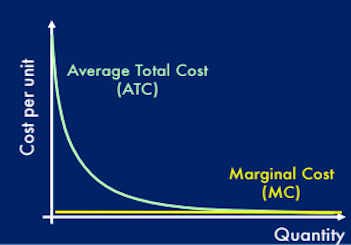
\includegraphics[width=.5\textwidth]{digitalCostCurve.PNG}
  \caption{Consumer Surplus \& Expenditure}
\end{figure}

\begin{remark}{Competition between Digital Companies}
  \begin{itemize}
    \item Due to low variable costs, companies with identical digital products will very quickly move prices to near-zero.
    \item New companies will struggle as fixed costs are high.
    \item Network effects \& switching costs make it hard for new companies.
  \end{itemize}
  Due to these \textit{barriers to entry} monopolies are common among digital companies. To succeed, a company needs to focus on product differentiation (i.e. innovation).
\end{remark}

\begin{remark}{Formats}
  Companies can make their software use \textit{Proprietary Formats}, meaning the files cannot be used by other software. This increases switching costs for customers.
  \par Using \textit{Industry-Wide Standards} allow a user's files to be shared between providers. This can increase the network effect, potentially attracting new customers. Here companies have a trade-off between having a large part of a small pie, or a small part of a large pie.
\end{remark}

\begin{remark}{How Standards Develop}
  \textit{Industry-Wide Standards} general develop in one of two ways
  \begin{enumerate}
    \item A \textit{single (major) player} sets a standard by opening up their proprietary format (e.g. PDF).
    \item A \textit{war} occurs between multiple standard setters. Generally detrimental to everyone involved.
    \item A \textit{negotiation} occurs between multiple standard setters. There is a risk that one party may pull out of the deal and use their own proprietary format.
  \end{enumerate}
\end{remark}

\subsection{Digital Monopolies}

\end{document}
